\begin{theorem}
    \begin{align*}
        &f: [a, b] \to \R \\
        &x_1, \ldots, x_n \\
        &P
    \end{align*}
    Si $f$  $n$ fois dérivable,  
    \[
        \forall x \in [a, b], \, \exists t \in ]a, b[, f(x) - P(x) = \omega_n(x)\frac{f^{(n)}(t)}{n!}
    \] 
\end{theorem}
\begin{preuve} du théorème (erreur)
    \par
    Soit x fixé des $[a, b] \setminus \{x_1, \ldots, x_n\}$
    \par
    On pose 
    \[
    F(t) = f(t) - P(t) - \frac{f(x) - P(x)}{\omega_n(t)}\omega_n(t)
    \] 
    $F$ est  $n$ fois dérivable et  $P$ annule aux  $n+1$ points  $x_1, \ldots, x_n, x$. D'apres le théorème Rolle (généralisé) 
    \[
        \exists t \in ]a, b[ \text{ tq } f^{(n)}(t) = 0
    \] 
    Or
    \[
        \underbrace{F^{(n)}(t)}_{= 0 \text{ par hyp}} = f^{(n)}(t) - \underbrace{P^{(n)}(t)}_{= 0 \text{ car } deg(P) < n} - \frac{f(x) - P(x)}{\omega_n(x)}n!
    \] 
    D'où
    \[
        f(x) - P(x) = \omega_N(x) \frac{f^{(n)}(t)}{n!}
    \] 
    Par ailleurs, si $x \in \{x_1, \ldots, x_n\}, \, f(x) - P(x) = 0$
    \[
    \omega_n(x) = (x - x_1)\ldots(x - x_n)
    \] 
\end{preuve}
\begin{preuve} corollaire
   \[
       |f(x) - P(x)| = |\omega_n(x)| \frac{|f^{(n)}(t)|}{n!}
   \]  
   comme $x, x_i \in [a, b]$, on a  $|x - x_i| \le b - a$ et $|f^{(n)}(t)| \le M$, on a:
   \[
   |f(x) - P(x) \le \frac{M}{n!}(b - a)^n
   \] 
\end{preuve}

\subsubsection{Evaluation efficace: formule barycentrique}
\begin{prop}
   On a 
   \begin{align*}
       P(x) &= \sum_{i=1}^{n} y_i \frac{\omega_n(x)}{(x - x_i)\omega_n'(x_i)}\\
            &= \frac{\sum_{i=1}^{n} \frac{1}{(x - x_i)\omega_n'(x_i)}y_i}{\sum_{i=1}^{n} \frac{1}{(x - x_i)\omega_n'(x_i)}}
   \end{align*}
\end{prop}
\begin{preuve}
   Comme 
   \[
   \omega_n(x) = \prod_{i=1}^{n} (x - x_i) \implies \omega_n'(x) = \sum_{i=1}^{n} \prod_{j=1 \quad j \neq 1}^{n} (x - x_j)  
   \] 
   D'où
   \[
   \omega_n'(x_i) = \prod_{j=1 \quad j \neq i}^{n} (x_i - x_j) \quad i = 1, \ldots, n
   \] 
   D'où 
   \[
   L_i(x) = \frac{\omega_n(x)}{x - x_i}\frac{1}{\omega_n'(x_i)}
   \] 
   Et 
   \begin{align*}
       \sum_{i=1}^{n} y_iL_i(x) &= \sum_{i=1}^{n} \frac{y_i}{(x - x_i)\omega_n'(x)}\omega_n(x)\\
                                &= \omega_n(x) \sum_{i=1}^{n} \frac{y_i}{(x - x_i)\omega_n'(x_i)}
   \end{align*}
   Or pour $P \equiv 1$ on a  $y_i = 1, i = 1, \ldots, n$, on a
   \[
   1 = \omega_n(x) \sum_{i=1}^{n} \frac{1}{(x - x_i)\omega_n'(x)}
   \] 
   D'où
   \[
       \omega_n(x) = \left(   \sum_{i=1}^{n} \frac{1}{(x - x_i)\omega_n'(x)}\right)^{-1}
   \] 
   Enfin,
   \[
   P(x) = \frac{\sum_{i=1}^{n} \frac{y_i}{(x - x_i)\omega_n'(x)}}{\sum_{i=1}^{n} \frac{1}{(x - x_i)\omega_n'(x)}}
   \] 
\end{preuve}
\begin{remark}
   \begin{enumerate}
       \item Attention: si $x = x_i, \, i = 1, \ldots, n$
       \item Exercice: calculer la complexité de cette formule et comparer à la première.
       \item Ajouter un nouveau point d'interpolation ablige à refaire tous les calculs.
   \end{enumerate} 
\end{remark}

\subsection{Méthode des différences divisées}
\subsubsection{Préliminaires: Interpolation de Neville}
\begin{lemma}
   Considérons $n$ points 2 à 2 distincts $x_1, \ldots, x_n$ et $n$ réels  $y_1, \ldots, y_n$. Pour $1 \le k \le l \le n$, posons $P_{x_k, \ldots, x_l}$ le polynôme d'interpolation aux points 
   \[
       (x_k, y_k) \ldots (x_l, y_l)
   \] 
   Nous avons
   \[
       P_{x_k, \ldots, x_l}(x) = \frac{(x - x_l)P_{x_l \ldots x_{l - 1}}(x) - (x - x_k)P_{x_{k+1}\ldots x_l}(x)}{x_k - x_l}
   \] 
   Schématiquement
   \[
       P(x) = \underbrace{x_k, \overbrace{x_{k+1}, \ldots, x_{l-1}}_{P_1}, x_l}^{P_2}
   \] 
   \[
   \frac{x - x_l}{x_k - x_l}P_1 + \frac{x - x_k}{x_l - x_k}P_2
   \] 
\end{lemma}

\subsubsection{Construction de l'intérpolation de Newton}
\begin{definition} (Polynôme de Newton)
    Soit $n \ge 1$ entier, $x_1, \ldots, x_n$ $n$ rééls 2 à 2 distincts. Les polynômes de Newton  $\omega_0, \ldots, \omega_n$ associés à ces points sont définis par
    \[
    \begin{cases}
        \omega_0 = 1\\
        \omega_j = (x - x_1) \ldots (x - x_j), \quad (1 \le j \le n)
    \end{cases}
    \] 
\end{definition}
\begin{remark}
    $\{\omega_j\}_{j = 1, \ldots, k}$ est une base de $\R_k[x]$    
    \begin{itemize}
        \item Ainsi le polynôme d'intérpolation de Lagrange associé aux points $(x_1, y_1) \ldots (x_n, y_n)$ s'écrit
            \[
            P = \sum_{k=0}^{n-1} \alpha_k\omega_k
            \] 
            où $\alpha_k$ sont solutions de 
             \[
            y_i = \sum_{k=0}^{n-1} \alpha_k\omega_k(x_i), \quad i = 1, \ldots, n
            \] 
    \end{itemize}
\end{remark}
On parle de développement de Newton du polyôme de Lagrange

\begin{definition}
    On appelle differences divisées d'ordre $j-1$ ($1 \le j \le n$) associées aux points $(x_1, y_1), \ldots, (x_i, y_i)$ les nombres $d_{i, j}$ ($i = j$ à $n$) définis par
    \begin{itemize}
        \item $d_{i, 1} = y_i \quad i = 1, \ldots, n$
        \item $d_{i, j} = \frac{d_{i, j-1} - d_{i-1,j-1}}{x_i - x_{i - j + 1}}$ \quad $j = 2$ à $n$, $i = j$ à $n$
    \end{itemize}
    Lorsque $y_i = f(x_i) \quad i = 1, \ldots, n$, $d_{i, j}$  est généralement noté $f[x_{j-i+1}, \ldots, x_{j-1}, x_j]$ et est appelé difference divisé d'ordre $j-1$ aux  $i$ points  $x_{j - i + 1}, \ldots, x_j$
\end{definition}
Python:
\begin{lstlisting}
def MatriceDifferencesDivisee(x, y):
    n = len(y)
    d = np.zeros((n, n))
    d[:, 0] = 1.0 * y
    for j in range(1, n):
        d[j:n, j] = (d[j:n, j-1] - d[j-1:n, j-1]) / (x[j:n] - x[0:n-j])
    return d
\end{lstlisting}
\begin{remark}
   \begin{itemize}
       \item Le "stencil" (squelette) est
           \begin{center}
              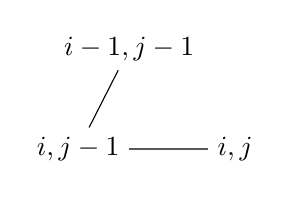
\begin{tikzpicture}
                  \node[above] (a) at (0, 1){$i-1, j-1$};
                  \node[left] (b) at (0, 0){$i, j-1$};
                  \node[right] (c) at (1, 0){$i, j$};
                  \draw (a) -- (b) -- (c);
              \end{tikzpicture} 
           \end{center}
        \item La hauteur de stencil est $j$
        \item Le support du stencil est  $[x_{i-j}, \ldots, x_{i}]$
   \end{itemize} 
\end{remark}
\begin{prop}
    On a $d_{j,j} = \alpha_{j-1}$  pour $j \in [1, \ldots, n]$, càd:
    \[
    P = \sum_{j=1}^{n} d_{j,j}\omega_{j-1}
    \] 
    Ainsi, pour calculer $P$ il suffit de connaître  $d_{j, j} \quad j = 1, \ldots, n$
\end{prop}

\subsubsection{Calcul efficace du polynôme}
\begin{prop}
   Soit donné $x_0, \ldots, x_n$ dés rééls 2 à 2 distincts. Soit $Q$ le polyôme défini par 
   \[
   Q(x) = a_0 + \sum_{i=1}^{n} a_i \prod_{j=1}^{i-1} (x - x_j) \equiv \sum_{i=0}^{n} a_i\omega_i(x) 
   \] 
   La suite des polynômes $Q_0, \ldots, Q_n$ définies par
   \[
   \begin{cases}
       Q_n = a_n\\
       Q_k = a_k + (x - x_k)Q_k \quad k = n-1, \ldots, 0
   \end{cases}
   \] 
   vérifie $Q_0 = Q$
\end{prop}
\begin{lstlisting}
def HornerNewton(d, x, xx):
    n = len(d)
    yy = 0 * xx + d[n-1]
    for i in range(n-2, -1, -1):
        yy = d[i] + (xx - x[i]) * yy
    return yy
\end{lstlisting}
\begin{lstlisting}
def DifferencesDivisees(x, y):
    d = MatriceDifferencesDivisee(x, y)
    a = np.diag(d)
    return a
\end{lstlisting}
